\section{Dati e Calcoli}
In questa sezione si deve raccogliere tutti i risultati che si sono ottenuti. Vanno bene foto, tabelle di dati e osservazioni personali. I dati sarebbe buono che vengano raccolti in tabella se sono in numero sufficiente. 
\'E anche vero che si possono unire le due sezioni dei dati per rendere più discorsivo il tutto.

In questa sezione si devono anche scrivere tutte le formule che si usano per i calcoli indicando cosa servono e le loro unità di misura.

Ci sono due modi per impostare le cose, nel primo modo si scrivono prima tutte le formule e poi dopo si svolgono i conti con i propri dati, oppure in alternativa, si scrive la formula e poi subito dopo il conto relativo. Se si sceglie di fare il secondo metodo si potrebbe usare una tabella

\textbf{Primo metododo:}
Le moli si trovano tramite la seguente formula:
\begin{equation}
   n=M[mol/L]\cdot V[L]=n [mol] 
   \label{eq:mol} %questo ti serve per citare le equazioni, in questa sezione non è molto utile ma nei cenni teorici ti può aiutare a scrivere meglio le frasi senza intortarti da solo
\end{equation}
E ora si svolge il calcolo sui propri dati, in questo caso aggiungo un "*" all'ambiente per togliere i numeri:
\begin{equation*}
   n=\frac{0.5\cdot 25}{1000}=0.0125 [mol] 
\end{equation*}
Si divide per  1000 percheè il volume è stato espresso in mL.

\textbf{Nel secondo modo invece:}
\begin{center}
    \begin{tabularx}{0.9\textwidth}{XcX}
    Formule & & Calcoli\\
    \midrule
    $n=M[mol/L]\cdot V[L]=n [mol] $ &$\rightarrow$& $ n=\frac{0.5\cdot 25}{1000}=0.0125 [mol] $\\
    $n=M[mol/L]\cdot V[L]=n [mol] $ &$\rightarrow$& $ n=\frac{0.5\cdot 25}{1000}=0.0125 [mol] $\\
    $n=M[mol/L]\cdot V[L]=n [mol] $ &$\rightarrow$& $ n=\frac{0.5\cdot 25}{1000}=0.0125 [mol] $\\
    $n=M[mol/L]\cdot V[L]=n [mol] $ &$\rightarrow$& $ n=\frac{0.5\cdot 25}{1000}=0.0125 [mol] $\\
    $n=M[mol/L]\cdot V[L]=n [mol] $ &$\rightarrow$& $ n=\frac{0.5\cdot 25}{1000}=0.0125 [mol] $\\
    \end{tabularx}
\end{center}
Bisogna trovare il modo per distanziare un po' il testo in verticale ma ci può stare.

\subsection{Dati sperimentali}
Vanno riportati \textit{tutti} i dati sperimentali, evidenziando se necessario, quelli "aberranti", cioè da scartare sulla base si un analisi statistica.
Laddove possibile, è bene raccogliere i dati sotto forma di tabelle.
\vspace{1ex}
\begin {center}
\begin{tabular}{c|c}
     Esperimento &  Risultato\\
     1 & 10\\
     2 & 15\\
     3 & ...
\end{tabular}
\end {center}

\subsection{Elaborazione dei dati}
(Se necessario anche grafica): riporta i calcoli effettuati a partire dai risultati sperimentali, indicando le relazioni matematiche utilizzate. L'elaborazione può consistere anche nella costruzione di diagrammi o grafici.
A volte essa prevede anche il trattamento statistico dei dati.

Plotting from data:
\begin{center}
\vspace{2ex}
\begin{figure}[!ht]
    \centering
    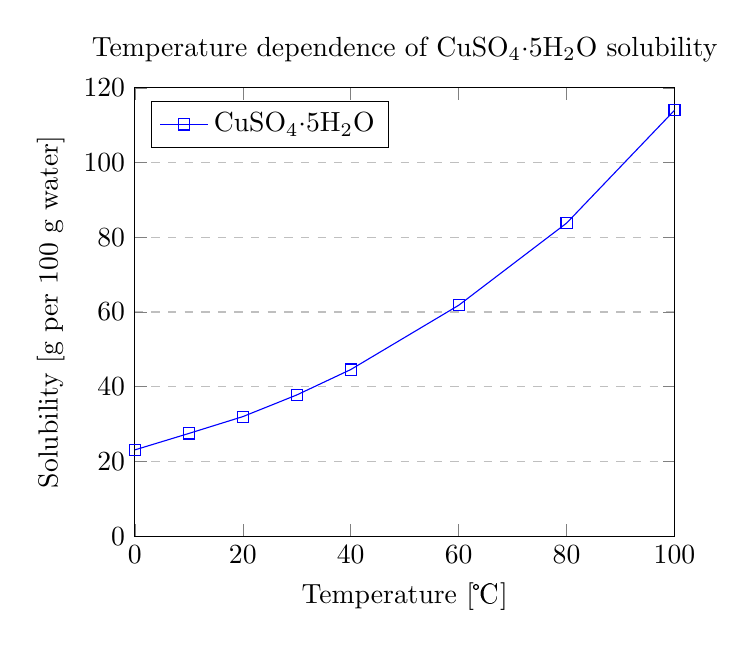
\begin{tikzpicture}
        \begin{axis}[
            title={Temperature dependence of CuSO\(_4\cdot\)5H\(_2\)O solubility},
            xlabel={Temperature [\textcelsius]},
            ylabel={Solubility [g per 100 g water]},
            xmin=0, xmax=100,
            ymin=0, ymax=120,
            xtick={0,20,40,60,80,100},
            ytick={0,20,40,60,80,100,120},
            legend pos=north west,
            ymajorgrids=true,
            grid style=dashed,
            ]

            \addplot[
                color=blue,
                mark=square,
                ]
                coordinates {
                (0,23.1)(10,27.5)(20,32)(30,37.8)(40,44.6)(60,61.8)(80,83.8)(100,114)
                };
                \legend{CuSO\(_4\cdot\)5H\(_2\)O}
                
            \end{axis}
        \end{tikzpicture}
    \caption{Grafico di solubilità del solfato di rame in base alla temperatura.}
    \label{plt:1}
\end{figure}

\end{center}
\newpage

